% 注意事项:编译两次,以确保目录、页码完整显示

\def\allfiles{}

\documentclass[14pt,a4paper,UTF8,twoside]{article}

% Formatting Packages ——————————————————————————————————————
\usepackage{multicol}
\usepackage{multirow}
\usepackage{enumitem}
\usepackage{indentfirst}
\usepackage[toc]{multitoc}

% Math & Physics Packages ————————————————————————————
\usepackage{amsmath, amsthm, amsfonts, amssymb}
\usepackage{setspace}
\usepackage{physics}
\usepackage{cancel}
\usepackage{nicefrac}
\usepackage{unicode-math} % 允许数学公式使用特定字体

% Image-related Packages —————————————————————————————
\usepackage{float} % 浮动体环境
\usepackage{subcaption} % 子图包
\usepackage{graphics, graphicx}
\usepackage{tikz, tikz-qtree}
\usepackage{mdframed}
\usepackage{lmodern}
\usetikzlibrary{arrows.meta}
\usetikzlibrary{shapes.geometric, arrows}
\tikzstyle{startstop} = [rectangle, rounded corners, minimum width=3cm, minimum height=1cm,text centered, draw=black, fill=red!30]
\tikzstyle{process} = [rectangle, minimum width=3cm, minimum height=1cm, text centered, draw=black, fill=blue!30]
\tikzstyle{arrow} = [thick,->,>=stealth]

\usepackage{pgfplots}
\pgfplotsset{compat=1.18}
\usepackage{xcolor}
\usepackage{fourier-orns}
\usepackage{lipsum}

% Colour Palette ——————————————————————————————————————
\definecolor{merah}{HTML}{F4564E}
\definecolor{merahtua}{HTML}{89313E}
\definecolor{biru}{HTML}{60BBE5}
\definecolor{birutua}{HTML}{412F66}
\definecolor{hijau}{HTML}{59CC78}
\definecolor{hijautua}{HTML}{366D5B}
\definecolor{kuning}{HTML}{FFD56B}
\definecolor{jingga}{HTML}{FBA15F}
\definecolor{ungu}{HTML}{8C5FBF}
\definecolor{lavender}{HTML}{CBA5E8}
\definecolor{merjamb}{HTML}{FFB6E0}
\definecolor{mygray}{HTML}{E6E6E6}
\definecolor{mygreen}{rgb}{0,0.6,0}
\definecolor{mymauve}{rgb}{0.58,0,0.82}

% Theorems ————————————————————————————————————————————
\usepackage{tcolorbox}
\usepackage{changepage}
\tcbuselibrary{skins,breakable,theorems}

\newcounter{hitung}
\setcounter{hitung}{\thesection}

\makeatletter
	% Proof 证明如下
	\def\tcb@theo@widetitle#1#2#3{\hbox to \textwidth{\textsc{\large#1}\normalsize\space#3\hfil(#2)}}
	\tcbset{
		theorem style/theorem wide name and number/.code={ \let\tcb@theo@title=\tcb@theo@widetitle},
		proofbox/.style={skin=enhancedmiddle,breakable,parbox=false,boxrule=0mm,
			check odd page, toggle left and right, colframe=black!20!white!92!hijau,
			leftrule=8pt, rightrule=0mm, boxsep=0mm,arc=0mm, outer arc=0mm,
			left=3mm,right=3mm,top=0mm,bottom=0mm, toptitle=0mm,
			bottomtitle=0mm,colback=gray!3!white!98!biru, before skip=8pt, after skip=8pt,
			before={\par\vskip-2pt},after={\par\smallbreak},
		},
	}
	\newtcolorbox{ProofBox}{proofbox}
	\makeatother
	
	\let\realproof\proof
	\let\realendproof\endproof
	\renewenvironment{proof}[1][Thoughts:]{\ProofBox\strut\textsc{#1}\space}{\endProofBox}
        \AtEndEnvironment{proof}{\null\hfill$\blacksquare$}
        % Definition 定义环境
	\newtcbtheorem[use counter=hitung, number within=section]{dfn}{定义}
	{theorem style=theorem wide name and number,breakable,enhanced,arc=3.5mm,outer arc=3.5mm,
		boxrule=0pt,toprule=1pt,leftrule=0pt,bottomrule=1pt, rightrule=0pt,left=0.2cm,right=0.2cm,
		titlerule=0.5em,toptitle=0.1cm,bottomtitle=-0.1cm,top=0.2cm,
		colframe=white!10!biru,
		colback=white!90!biru,
		coltitle=white,
		shadow={1.3mm}{-1.3mm}{0mm}{gray!50!white}, % 添加阴影
        coltext=birutua!60!gray, title style={white!10!biru}, rbefoe skip=8pt, after skip=8pt,
		fonttitle=\bfseries,fontupper=\normalsize}{dfn}

	% 答题卡
	\newtcbtheorem[use counter=hitung, number within=section]{ans}{解答}
	{theorem style=theorem wide name and number,breakable,enhanced,arc=3.5mm,outer arc=3.5mm,
		boxrule=0pt,toprule=1pt,leftrule=0pt,bottomrule=1pt, rightrule=0pt,left=0.2cm,right=0.2cm,
		titlerule=0.5em,toptitle=0.1cm,bottomtitle=-0.1cm,top=0.2cm,
		colframe=white!10!biru,
		colback=white!90!biru,
		coltitle=white,
		shadow={1.3mm}{-1.3mm}{0mm}{gray!50!white}, % 添加阴影
        coltext=birutua!60!gray, title style={white!10!biru}, before skip=8pt, after skip=8pt,
		fonttitle=\bfseries,fontupper=\normalsize}{ans}

	% Axiom
	\newtcbtheorem[use counter=hitung, number within=section]{axm}{公理}
	{theorem style=theorem wide name and number,breakable,enhanced,arc=3.5mm,outer arc=3.5mm,
		boxrule=0pt,toprule=1pt,leftrule=0pt,bottomrule=1pt, rightrule=0pt,left=0.2cm,right=0.2cm,
		titlerule=0.5em,toptitle=0.1cm,bottomtitle=-0.1cm,top=0.2cm,
		colframe=white!10!biru,colback=white!90!biru,coltitle=white,
		shadow={1.3mm}{-1.3mm}{0mm}{gray!50!white!90}, % 添加阴影
        coltext=birutua!60!gray,title style={white!10!biru},before skip=8pt, after skip=8pt,
		fonttitle=\bfseries,fontupper=\normalsize}{axm}
 
	% Theorem
	\newtcbtheorem[use counter=hitung, number within=section]{thm}{Warning}
	{theorem style=theorem wide name and number,breakable,enhanced,arc=3.5mm,outer arc=3.5mm,
		boxrule=0pt,toprule=1pt,leftrule=0pt,bottomrule=1pt, rightrule=0pt,left=0.2cm,right=0.2cm,
		titlerule=0.5em,toptitle=0.1cm,bottomtitle=-0.1cm,top=0.2cm,
		colframe=white!10!merah,colback=white!75!pink,coltitle=white, coltext=merahtua!80!merah,
		shadow={1.3mm}{-1.3mm}{0mm}{gray!50!white!90}, % 添加阴影
		title style={white!10!merah}, before skip=8pt, after skip=8pt,
		fonttitle=\bfseries,fontupper=\normalsize}{thm}
	
	% Proposition
	\newtcbtheorem[use counter=hitung, number within=section]{prp}{Advantages}
	{theorem style=theorem wide name and number,breakable,enhanced,arc=3.5mm,outer arc=3.5mm,
		boxrule=0pt,toprule=1pt,leftrule=0pt,bottomrule=1pt, rightrule=0pt,left=0.2cm,right=0.2cm,
		titlerule=0.5em,toptitle=0.1cm,bottomtitle=-0.1cm,top=0.2cm,
		colframe=white!10!hijau,colback=white!90!hijau,coltitle=white, coltext=hijautua!80!brown,
		shadow={1.3mm}{-1.3mm}{0mm}{gray!50!white}, % 添加阴影
		title style={white!10!hijau}, before skip=8pt, after skip=8pt,
		fonttitle=\bfseries,fontupper=\normalsize}{prp}


	% Example
	\newtcolorbox[use counter=hitung, number within=section]{cth}[1][]{breakable,
		colframe=white!10!jingga, coltitle=white!90!jingga, colback=white!85!jingga, coltext=black!10!brown!50!jingga, colbacktitle=white!10!jingga, enhanced, fonttitle=\bfseries,fontupper=\normalsize, attach boxed title to top left={yshift=-2mm}, before skip=8pt, after skip=8pt,
		title=Tips~\thetcbcounter \ \ #1}

	% Catatan/Note
	\newtcolorbox{ctt}[1][]{enhanced, 
		left=4.1mm, borderline west={8pt}{0pt}{white!10!kuning}, 
		before skip=6pt, after skip=6pt, 
		colback=white!85!kuning, colframe= white!85!kuning, coltitle=orange!60!kuning!25!brown, coltext=orange!60!kuning!25!brown,
		fonttitle=\bfseries,fontupper=\normalsize, before skip=8pt, after skip=8pt,
		title=\underline{Notice}  #1}
	
	% Komentar/Remark
	\newtcolorbox{rmr}[1][]{
		,arc=0mm,outer arc=0mm,
		boxrule=0pt,toprule=1pt,leftrule=0pt,bottomrule=5pt, rightrule=0pt,left=0.2cm,right=0.2cm,
		titlerule=0.5em,toptitle=0.1cm,bottomtitle=-0.1cm,top=0.2cm,
		colframe=white!10!kuning,colback=white!85!kuning,coltitle=white, coltext=orange!60!kuning,
		fonttitle=\bfseries,fontupper=\normalsize, before skip=8pt, after skip=8pt,
		title=Question  #1}

\usepackage{booktabs} % 表格库
\usepackage{titlesec} % 标题库
\usepackage{fancyhdr} % 页眉页脚库
\usepackage[sorting=none]{biblatex}
\usepackage{array}
\usepackage{longtable}
\usetikzlibrary{positioning, arrows.meta}
\addbibresource{references.bib} % 指定你的.bib文件名称

\date{} % 留空,以让编译时去除日期

%———————————————注意事项—————————————————%

% 1、如果编译显示失败,但没有错误信息,就是 filename.pdf 正在被占用
% 2、在文件夹中的终端使用 Windows > xelatex filename.tex 也可编译

%—————————————华东师范大学———————————————%

% 论文制作时须加页眉,页眉从中文摘要开始至论文末
% 偶数页码内容为:华东师范大学硕士学位论文,奇数页码内容为学位论文题目

%————————定义 \section 的标题样式————————%

% 注意:\chapter 等命令,内部使用的是 \thispagestyle{plain} 的排版格式
% 若需要自己加上页眉,实际是在用 \thispagestyle{fancy} 的排版格式
% 加上下面这一段指令,就能够让 \section 也使用 fancy 的排版格式
% 本质就是让目录、第一页也能够显示页眉、页脚

\fancypagestyle{plain}{
  \pagestyle{fancy}
}

\title{华东师范大学软件学院课程作业} % 模板
\titleformat{\section}
    {\normalfont\bfseries\Large} % 字体大小、字体系列(\bfseries 为加粗)
    {\thesection}{1em}{}

% ———————————设置章节的中文格式———————————%
\renewcommand\thesection{\chinese{section} \hspace{0pt}}
\renewcommand\thesubsection{\arabic{subsection} \hspace{0pt}}
% \renewcommand\thesubsubsection{\alph{subsubsection} \hspace{0pt}} % 字母编号
% \hspace{0pt} 是为了确保在章节编号和章节题目之间不要有空格,使得排版更为美观
    
%—————————————页面基础设置———————————————%

\usepackage{geometry}
\geometry{left=10mm, right=10mm, top=20mm, bottom=20mm}

%————————————设置页眉、页脚——————————————%

\pagestyle{fancy} % 设置 plain style 的属性

% 设置页眉

\fancyhead[RE]{\footnotesize \leftmark} % Right Even 偶数页右侧显示章名 \leftmark 最高级别章名
\fancyhead[LO]{\footnotesize \rightmark} % Left Odd 奇数页左侧显示节名 \rightmark 第二级别节名
\fancyhead[C]{华东师范大学软件学院课程作业} % Center 居中显示
\fancyhead[LE,RO]{~\thepage~} % 在偶数页的左侧,奇数页的右侧显示页码
\renewcommand{\headrulewidth}{1.2pt} % 页眉与正文之间的水平线粗细

% 设置页脚:在每页的右下脚以斜体显示书名

\fancyfoot[RO,RE]{\it Homework 6 By \LaTeX} % 使用意大利斜体显示
\renewcommand{\footrulewidth}{0.5pt} % 页脚水平线宽度

%——————设置页码:在底部居中显示页码———————%

\usepackage{lastpage} % 页码数库
\pagestyle{fancy}
\fancyfoot[C]{\kaishu 第 \thepage 页 \ 共 \pageref{LastPage} 页} % LastPage 需要二次编译以获取总页数

%——————————————代码块设置———————————————%

\usepackage{listings} % 代码块包
\lstset {
    backgroundcolor=\color{white},   % choose the background color; you must add \usepackage{color} or \usepackage{xcolor}
    basicstyle=\footnotesize,        % the size of the fonts that are used for the code
    breakatwhitespace=false,         % sets if automatic breaks should only happen at whitespace
    breaklines=true,                 % sets automatic line breaking
    captionpos=bl,                   % sets the caption-position to bottom
    commentstyle=\color{mygreen},    % comment style
    deletekeywords={...},            % if you want to delete keywords from the given language
    escapeinside={\%*}{*},           % if you want to add LaTeX within your code
    extendedchars=true,              % lets you use non-ASCII characters; for 8-bits encodings only, does not work with UTF-8
    frame=single,                    % adds a frame around the code
    keepspaces=true,                 % keeps spaces in text, useful for keeping indentation of code (possibly needs columns=flexible)
    keywordstyle=\color{blue},       % keyword style
    % language=Python,               % the language of the code
    morekeywords={*,...},            % if you want to add more keywords to the set
    numbers=left,                    % where to put the line-numbers; possible values are (none, left, right)
    numbersep=5pt,                   % how far the line-numbers are from the code
    numberstyle=\tiny\color{mygray}, % the style that is used for the line-numbers
    rulecolor=\color{black},         % if not set, the frame-color may be changed on line-breaks within not-black text (e.g. comments (green here))
    showspaces=false,                % show spaces everywhere adding particular underscores; it overrides 'showstringspaces'
    showstringspaces=false,          % underline spaces within strings only
    showtabs=false,                  % show tabs within strings adding particular underscores
    stepnumber=1,                    % the step between two line-numbers. If it's 1, each line will be numbered
    stringstyle=\color{orange},      % string literal style
    tabsize=2,                       % sets default tabsize to 2 spaces
    % title=Python Code              % show the filename of files included with \lstinputlisting; also try caption instead of title
}

% 注释掉的部分用于后续插入代码,参数可调整,格式如下:

% 1、直接插入
% \begin{lstlisting}[language = ? , title = { ? } ]
%       Your code here.
% \end{lstlisting}

% 2、文件插入
% \lstinputlisting[language = C , title = ?.c] {filename.c}

%———————————————字体设置————————————————%

\usepackage{fontspec} % 允许设置字体
\usepackage[utf8]{inputenc}
\usepackage{ctex}
\usepackage{pifont}
\linespread{1.2}
% \setCJKmainfont{SimSun} % 设置正文罗马族的 CJK 字体
\renewcommand{\texttt}[1]{\textcolor{blue}{\ttfamily #1}}

%———————————————超链接设置——————————————%

\usepackage[hidelinks]{hyperref}
\hypersetup{
    pdfstartview=FitH, % 设置PDF文档打开时的初始视图为页面宽度适应窗口宽度(即页面水平适应)
    CJKbookmarks=true, % 用对CJK(中文、日文、韩文)字符的书签支持,确保这些字符在书签中正确显示
    bookmarksnumbered=true, % 书签带有章节编号。这对有章节编号的文档很有用
    bookmarksopen=true, % 文档打开时,书签树是展开的,方便查看所有书签
    colorlinks, % 启用彩色链接。这样,链接在PDF中会显示为彩色,而不是默认的方框
    pdfborder=001, % 设置PDF文档中链接的边框样式。001 表示链接周围没有边框,仅在单击时显示一个矩形
    linkcolor=blue, % 设置文档内部链接(如目录中的章节链接)的颜色为蓝色
    anchorcolor=blue, % 设置锚点链接(即目标在同一文档内的链接)的颜色为蓝色
    citecolor=blue, % 设置引用(如文献引用)的颜色为蓝色
}

%————————————导言区结束,进入正文部分————————————%

%——————————————————————————————————————%

\begin{document}

\maketitle

\begin{center} % \extracolsep{\fill} 拉伸到页面最大宽度前,保证居中显示

  \begin{tabular*}{\textwidth}{@{\extracolsep{\fill}} l  l  l }
    \hline
    课程名称:计算机网络 &  年级:2023级本科  &  姓名:张梓卫 \\
    作业主题:第六章作业 & 学号:10235101526 & 作业日期:2024/12/31 \\
    指导老师:刘献忠 & 组号: \\
    \hline
  \end{tabular*}

\end{center}

% \tableofcontents % 目录也需要二次编译

\section{6.1}

\subsection*{题目}

In our example transport primitives of Fig. 6-2, LISTEN is a blocking call. Is this strictly necessary? If not, explain how a nonblocking primitive could be used. What advantage would this have over the scheme described in the text?

\begin{figure}[H]
    \centering
    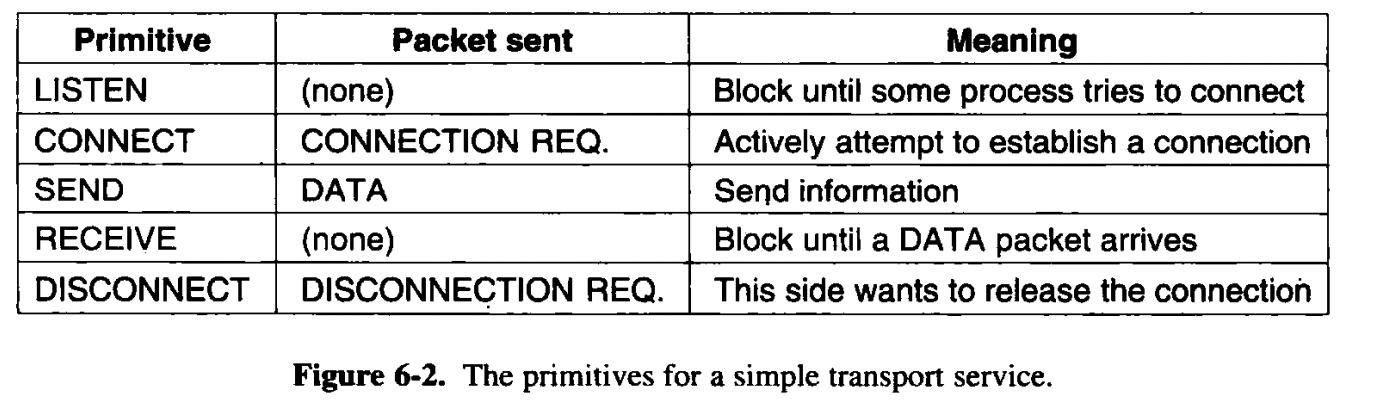
\includegraphics[width=0.57\textwidth]{lec6/6-2.png}
    \label{fig:6-2}
\end{figure}

\subsection*{解答}

LISTEN作为阻塞调用并非严格必要。事实上,LISTEN可以被设计为非阻塞调用。在非阻塞方案中,LISTEN调用仅表示建立新连接的意愿,并立即返回。当有连接尝试时,程序可以通过信号通知或回调机制处理连接请求。例如,可以执行“OK”或“REJECT”操作来接受或拒绝连接。

\begin{prp}{}{}
\begin{itemize}
    \item \textbf{提高效率}:允许程序在等待连接时继续执行其他任务,例如处理日志或管理其他网络活动,从而更高效地利用系统资源。
    \item \textbf{增强灵活性}:开发者可以灵活设计程序逻辑,而不受阻塞机制的限制。
    \item \textbf{避免死锁风险}:在某些复杂的多线程或多进程环境中,非阻塞操作可以减少死锁或资源竞争的风险。
\end{itemize}
\end{prp}

\begin{thm}{}{}
\begin{itemize}
    \item \textbf{实现复杂度增加}:非阻塞模式需要额外的轮询或事件通知机制,增加了开发和维护的复杂性。
    \item \textbf{潜在性能问题}:轮询可能导致系统开销增加,特别是在高负载场景中。如果使用事件驱动机制,则需要支持底层事件通知接口。
\end{itemize}
\end{thm}

非阻塞LISTEN原语适用于需要同时处理多项任务的复杂应用程序,能够提高系统的并发能力和灵活性。

若是对于简单的单任务程序,阻塞LISTEN可能更容易实现和维护。

\section{6.2}

\subsection*{题目}

In the underlying model of Fig. 6-4, it is assumed that packets may be lost by the network layer and thus must be individually acknowledged. Suppose that the network layer is 100 percent reliable and never loses packets. What changes, if any, are needed to Fig. 6-4?

\begin{figure}[H]
    \centering
    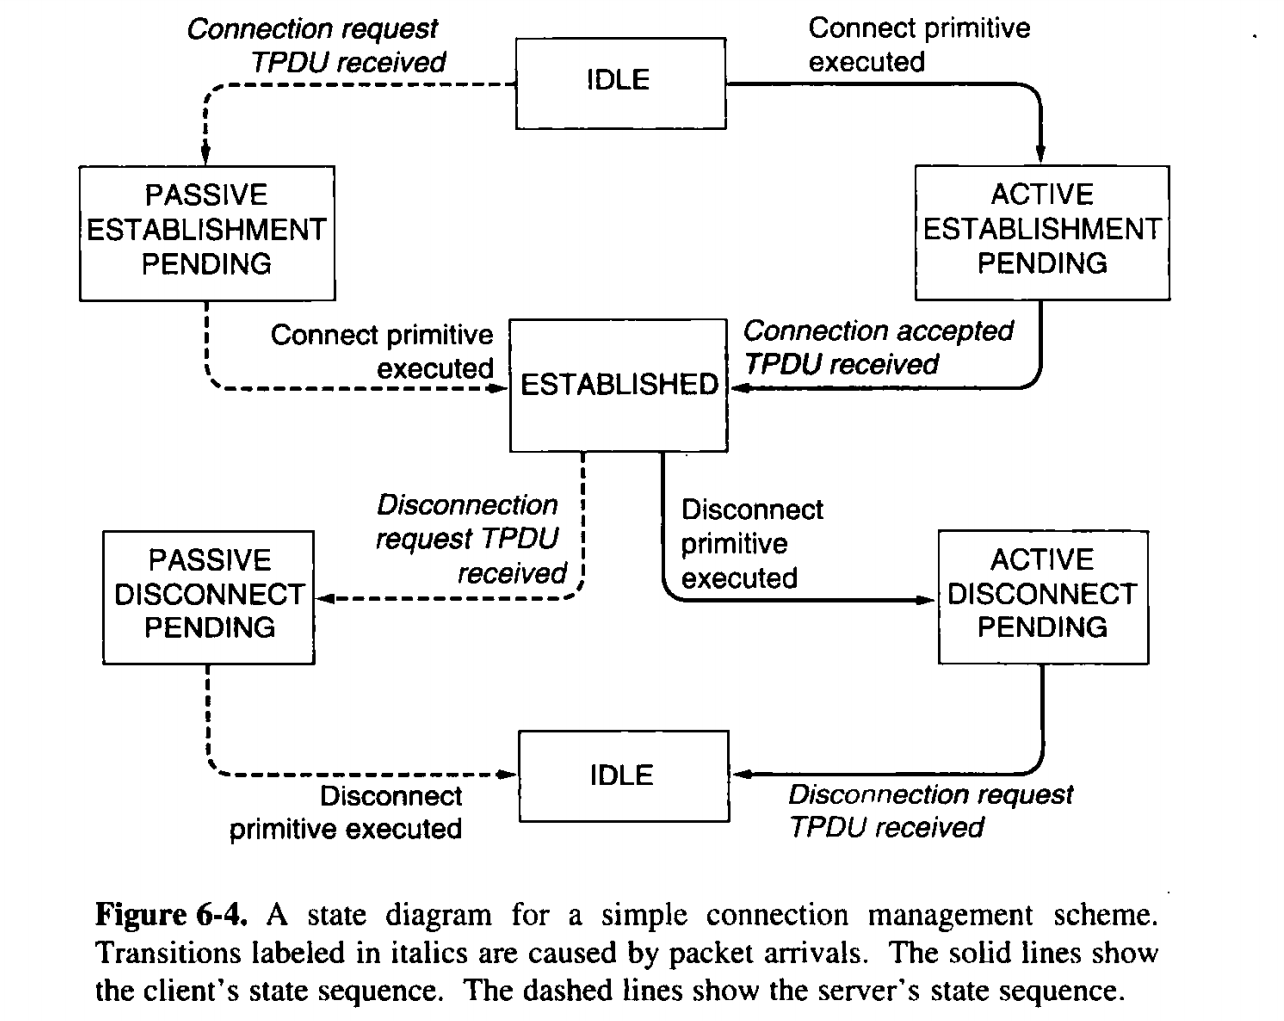
\includegraphics[width=0.45\textwidth]{lec6/6-4.png}
    \label{fig:6-4}
\end{figure}

\subsection*{解答}

如果网络层是100%可靠且从不丢失分组,那么在图6-4中,不再需要对每个分组进行单独确认。
可以简化协议,省略确认机制,或者使用更高效的确认方法,如累积确认。

设计可以做如下调整:

\begin{cth}
\begin{itemize}
    \item 取消对每个分组的单独确认:在网络层100%可靠的情况下,发送方可以假设分组一定会被成功送达,无需为每个分组单独发送确认信息。可以简化协议,直接省略确认机制。
    \item 直接建立连接状态:由于网络层可靠性保证,连接可以直接从`PASSIVE ESTABLISHMENT PENDING`状态跳转到`ESTABLISHED`状态,因为可以确认对方肯定能收到消息。无需等待额外的确认即可建立连接。
    \item 保留断开连接的PENDING状态:虽然网络层可靠,但在断开连接时,收到客户端的断开请求只意味着不会再接收来自客户端的数据包。此时,服务器仍可能有未发送完的数据包需要发给客户端,因此在断开连接时仍需要保持`PENDING`状态以完成数据传输。
    \item 使用累积确认或滑动窗口机制:如果仍需提高传输效率,可以使用累积确认来一次确认多个分组的接收情况,或者使用滑动窗口机制,在等待ACK之前允许发送多个分组,提高整体传输效率。
\end{itemize}
\end{cth}

\section{6.3}

\subsection*{题目}

Why does the maximum packet lifetime, T, have to be large enough to ensure that not only the packet but also its acknowledgements have vanished?

\subsection*{解答}

为了理解这个问题,首先需要明确三次握手过程是如何解决延迟或重复引发的问题。

\begin{itemize}
    \item 主机1发送连接请求时,选择一个序列号$x$,并向主机2发送一个包含该序列号的连接请求TPDU;
    \item 主机2收到请求后,回应该连接请求的TPDU,确认$x$,并声明自己选用的初始序列号$y$;
    \item 最后,主机1在其发送的第一个数据TPDU中确认主机2所选择的初始序列号$y$。
\end{itemize}

\begin{ctt}
当出现延迟的重复控制TPDU时,例如,一个来自于已关闭连接的延迟重复连接请求(\textit{Connection Request})TPDU可能在主机1毫不知情的情况下被主机2接收到,这会引发问题:
\begin{itemize}
    \item 主机2会向主机1发送一个接受连接的TPDU(\textit{Connection Accepted})来响应该连接请求;
    \item 然而,这个“接受连接”的TPDU的真正目的是主机2确认建立一个新的连接,而不是响应旧的连接请求。
\end{itemize}

关键在于主机2需要使用一个从主机2到主机1交互的初始序列号$y$,这样可以确保该序列号所对应的旧TPDU或ACK已经不再存在于网络中。否则,可能会导致主机1对延迟的TPDU产生误解,从而试图建立新的连接。
\end{ctt}

最糟糕的情况是延迟的“连接请求”与“连接接受”的确认响应都在网络中存活。如果一个重发的分组到达,并且包含一个旧的序列号时:
\begin{itemize}
    \item 如果在网络中还有旧的分组或ACK,可能会混淆当前的连接过程,甚至破坏三次握手的正常工作。
    \item 错误的解析可能会导致故障性连接,从而引发难以定位的问题。
\end{itemize}

因此,最大分组寿命$T$必须足够大,以确保不仅数据分组本身已经从网络中消失,其对应的确认分组(ACK)也已经完全消失。这是为了避免由于分组或确认分组的延迟导致的混淆,例如新分组与旧确认分组的混淆,或者导致重复确认的错误解释。只有这样,才能确保协议的正确性,避免因旧分组或确认分组的存在而引发的传输错误,从而保证三次握手及连接管理的可靠性。

\section{6.4}

\subsection*{题目}

Discuss the advantages and disadvantages of credits versus sliding window protocols.

讨论信用与滑动窗口协议的优缺点。

\subsection*{解答}

\subsubsection*{滑动窗口协议}

\begin{prp}{}{}
    优点:滑动窗口协议实现较为简单,只需要管理窗口边界的一组参数(即窗口起始位置和结束位置),无需复杂的额外参数。
    不仅如此,其可靠性也较强,具体体现在可以连续发送多个分组,同时确保分组按序到达,避免了信用机制中窗口增加和减少时,可能出现分组乱序的问题。    
\end{prp}

\begin{thm}{}{}
    缺点:滑动窗口协议的灵活性较差,因为窗口大小的调整较为固定,无法根据接收方的具体缓冲区状态动态管理。
    在某些情况下,窗口资源可能未被充分利用,或导致传输效率降低。
\end{thm}

\subsubsection*{信用机制协议}

\begin{prp}{}{}
    优点:信用机制允许动态管理缓冲区的使用。接收方可以根据自身缓冲区的状况,为发送方分配适当的信用额度,避免发送方发送过多数据导致接收方缓冲区溢出。
    信用机制将缓冲区的动态管理与分组确认机制分离开,使得协议更加灵活。
\end{prp}

\begin{thm}{}{}
    缺点:信用机制需要额外维护和管理信用额度,这增加了协议的实现复杂性。
    还有一点是,信用额度信息的传递可能需要额外的通信开销。
\end{thm}

\section{6.5}

\subsection*{题目}

Why does UDP exist? Would it not have been enough to just let user processes send raw IP packets?

\subsection*{解答}

仅仅让用户进程发送原始IP数据包当然远远不够。

IP 数据包仅包含目标计算机的 IP 地址,无法识别具体的目标进程。

UDP 的存在不仅解决了IP分组无法区分目标进程的问题,还通过引入端口号和提供简单的传输层接口,使开发者能够专注于应用逻辑,而无需处理底层网络层的复杂性。相比直接发送IP分组,UDP提升了安全性、灵活性和标准化管理能力。

\begin{ctt}
UDP 提供一种简单、无连接的传输层协议,允许应用程序在不建立连接、无需保证可靠性或顺序的情况下发送数据报。相比让用户进程直接发送原始IP分组,UDP简化了传输过程,减少了协议开销,并提供了必要的接口和功能,使应用程序能够专注于自身逻辑而无需处理传输层的复杂性。此外,直接发送原始IP分组可能带来安全风险,且缺乏标准化的错误处理和流量控制机制,而UDP则通过标准化的接口和功能提供了更好的安全性和可管理性。
\end{ctt}

\section{6.6}

\subsection*{题目}

Suppose that the TCP congestion window is set to 18 KB and a timeout occurs. How big will the window be if the next four transmission bursts are all successful? Assume that the maximum segment size is 1 KB.

\subsection*{解答}

在TCP协议中,当发生超时时,拥塞窗口(cwnd)会被重置为1个最大报文段(MSS),并进入慢启动(Slow Start)阶段。此时,cwnd会从1 KB开始,逐渐按指数增长。假设MSS为1 KB,具体过程如下:

   \begin{itemize}
       \item cwnd被重置为1 KB。
       \item 阈值(ssthresh)被重置为 $ \text{18 KB}/2 = 9 \text{ KB}$。
   \end{itemize}

\begin{ans}{}{}
\subsubsection*{慢启动过程}
   \begin{itemize}
       \item \textbf{第1次传输成功}:cwnd增加到2 KB(发送1个分组)。
       \item \textbf{第2次传输成功}:cwnd增加到4 KB(发送2个分组)。
       \item \textbf{第3次传输成功}:cwnd增加到8 KB(发送4个分组)。
       \item \textbf{第4次传输成功}:cwnd理论上增加到16 KB(发送8个分组)。
   \end{itemize}

\subsubsection*{阈值限制}
   \begin{itemize}
       \item 由于阈值为9 KB,当cwnd达到或超过阈值后,增长进入拥塞避免阶段,在这种情况下,cwnd不能超过阈值。
   \end{itemize}

\end{ans}

因此,在经过四次成功的传输后,拥塞窗口的大小将增长至9 KB(受到阈值的限制)。

\section{6.7}

\subsection*{题目}

A TCP machine is sending full windows of 65,535 bytes over a 1-Gbps channel that has a 10-msec one-way delay. What is the maximum throughput achievable? What is the line efficiency?

\subsection*{解答}

\begin{ans}{}{}

    TCP窗口大小为 $65,535$ 字节。
    
    最大吞吐量可以通过窗口大小除以RTT来计算:
    \[
    \text{吞吐量} = \frac{\text{窗口大小}}{\text{RTT}} = \frac{65,535 \, \text{字节}}{0.02 \, \text{s}} = 3,276,750 \, \text{字节/秒} \approx 26.21 \, \text{Mbps}
    \]
    
    \[
    \text{线路效率} = \frac{\text{最大吞吐量}}{\text{带宽}} = \frac{26.21 \, \text{Mbps}}{1000 \, \text{Mbps}} = 2.62\%
    \]
    
    故最大吞吐量约为 $26.21$ Mbps,线路效率约为 $2.62\%$。
    \end{ans}

\section{6.8}

\subsection*{题目}

In a network whose max segment is 128 bytes, max segment lifetime is 30 sec, and has 8-bit sequence numbers, what is the maximum data rate per connection?

\subsection*{解答}

\begin{ans}{6.8}{6.8}
发送方最多可发送255个分段(由于序列号为8位,共有256个序列号,从0到255),因此:

\[
\text{最大数据量} = 255 \, \text{段} \times 128 \, \text{bytes/段} = 32,640 \, \text{bytes}
\]

分组的最大生命周期为30秒,因此最大数据速率为:

\[
\text{最大数据速率} = \frac{32,640 \, \text{bytes}}{30 \, \text{s}} \approx 1,088 \, \text{bytes/s}
\]

换算为比特:

\[
1,088 \, \text{bytes/s} \times 8 \, \text{bits/bytes} = 8,704 \, \text{bits/s}
\]

因此,每个连接的最大数据速率为 8,704 bps。
\end{ans}

\section{6.9}

\subsection*{题目}

A CPU executes instructions at the rate of 1000 MIPS. Data can be copied 64 bits at a time, with each word copied costing 10 instructions. If an incoming packet has to be copied four times, can this system handle a 1-Gbps line? For simplicity, assume that all instructions, even those instructions that read or write memory, run at the full 1000-MIPS rate.

\subsection*{解答}

\begin{ans}{}{}
每次复制 64 bits(8 字节)数据需要 10 条指令,复制四次总共需要 40 条指令:
\[
\text{每字节的指令数} = \frac{40}{8} = 5 \, \text{指令/字节}
\]

CPU 每秒执行 \( 1000 \times 10^6 \) 条指令,处理数据速率为:
\[
\text{数据速率} = \frac{1 \times 10^9 \, \text{指令/秒}}{5 \, \text{指令/字节}} = 200 \, \text{MB/s} = 1600 \, \text{Mbps}
\]

目标数据速率为 1 Gbps,因此:
\[
1600 \, \text{Mbps} > 1000 \, \text{Mbps}
\]

结论:该系统可以处理 1 Gbps 的网络连接。
\end{ans}

\section{6.10}

\subsection*{题目}

To get around the problem of sequence numbers wrapping around while old packets still exist, one could use 64-bit sequence numbers. However, theoretically, an optical fiber can run at 75 Tbps. What maximum packet lifetime is required to make sure that future 75-Tbps networks do not have wraparound problems even with 64-bit sequence numbers? Assume that each byte has its own sequence number, as TCP does.

\subsection*{解答}

\begin{ans}{6.10}{6.10}

序列号空间的大小为 \( 2^{64} \) 字节,这相当于约 \( 2 \times 10^{19} \) 字节。

假设网络以75 Tbps的速率传输,则每秒消耗的序列号数量为:

\[
75 \, \text{Tbps} = 75 \times 10^{12} \, \text{bits/second}
\]

转换为字节速率:

\[
\frac{75 \times 10^{12}}{8} = 9.375 \times 10^{12} \, \text{bytes/second}
\]

传输完 \( 2^{64} \) 字节所需的时间为:

\[
T = \frac{2^{64}}{9.375 \times 10^{12}} \approx \frac{1.844 \times 10^{19}}{9.375 \times 10^{12}} \approx 1,962,653 \, \text{seconds} \approx 22.7 \, \text{days}
\]

最大分组寿命应小于约22.7天,以确保不会出现序列号环绕问题。

\textbf{总结}:在未来75 Tbps的网络中,使用64位序列号可以有效避免序列号环绕问题,即使传输速率非常高。最大分组寿命的限制为约22.7天,这在实际中是一个非常宽裕的限制条件。

\end{ans}

\end{document}